\chapter{Artifact}

In this chapter, the context, dependencies, architecture, used technologies and testing are presented. Design decisions, implementation alternatives and resulting consequences are introduced and discussed along the other topics.


TODOS:
discussion of the design choices  a set of arguments on the final design choice



\section{System Context}

The reimbursement-tool interacts with several user types as well as external software systems. In this section, these actors and software systems are introduced and resulting dependencies outlined.

\subsection{Actors}

The context diagram (see figure \ref{fig:context-diagram}) describes the relationships between the system and its users:
\textit{Expense Creators}, in short creators, such as assistants, professors and the administrative employees can create, view and print expenses. However, they are only allowed to modify their own expenses while they are in the draft state i.e have not been submitted to the \textit{Expense Creators} manager yet.  \textit{Managers}, such as professors, the department manager, the head of institute and the \textit{Finance administration} are able to \textit{reject expenses} and send them back to the \textit{Expense Creators}. Besides rejecting expenses, they are also able to modify them. Moreover, \textit{Managers} have also to provide for each expense a project description. \textit{Finance administrators} can additionally to the \textit{managers} aggregate statistics, search for certain expenses and reset expenses that are stuck in the process (e.g. when a manager would have to sign the expense but left the IFI). \textit{Guests} are allowed to view specific expenses and related expense-items too. However, they need the 32-character long internal expense \textit{Uid} to gain access to the expense's details. The \textit{Uid} is added on the printed expense document (see appendix \ref{sec:app-pdf}).

\subsection{Services and Dependencies}
The following sub chapters explain what interfaces to external service providers exist.

\subsubsection{IFI LDAP Server}
The reimbursement-tool fetches user-data from the IFI LDAP server (see figure \ref{fig:context-diagram}) and stores it in the reimbursement-database. By being able to reuse the existing LDAP credentials, the user gets a comfortable way to login and ensures at the same time that only authenticated users gain access to the system. Furthermore, the user's current roles and the user's manager are assigned automatically. If there is no manager specified in the LDAP, a warning is shown to the user. For details about how to adjust the LDAP settings please refer to appendix \ref{subsubsec:ldap}.

\begin{figure}[H]
	\centering
	\fbox{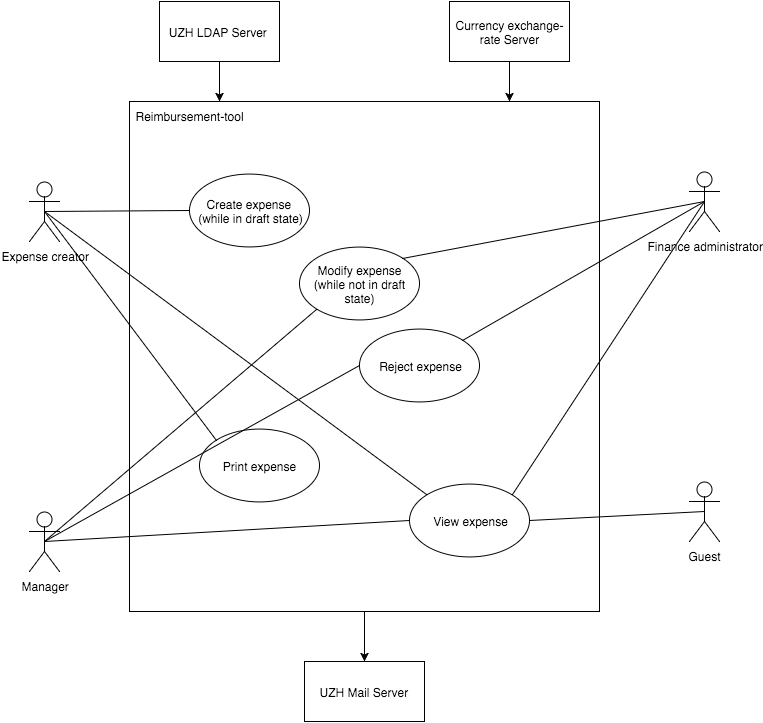
\includegraphics[width=0.80\textwidth]{context-diagram}}
	\caption{System context: Context diagram}
	\label{fig:context-diagram}
\end{figure}

\subsubsection{Currency exchange-rate Server}
Often expenses accrue in foreign currencies but are paid back in CHF. To provide the user with a handy but still accurate way to calculate the historically accurate amount that has to be charged back, the reimbursement tool integrates a currency-exchange-rate-service. We decided to use \textit{fixer.io} \cite{fixer} because it is free, updated daily, provides low response times and a high availability. While the \textit{European Central Bank(ECB)}\cite{ecb} is used as data source, \textit{fixer.io} provides a query-able web-service for it. Currently, the reimbursement-tool calls the API every time an exchange-rate is needed. For example if the user specifies the amount of a receipt in a foreign currency. Since the API is called by our reimbursement-server, any cheating regarding exchange rates is prevented.

\subsubsection{UZH Mail Server}
To notify users about actions that need their attention, the reimbursement-tool implements a notification algorithm. As soon as a new action has to be taken, the notification service adds the user's e-mail address to the e-mailing list. Emails are sent out only three times a day (8am, 12pm and 5pm). At this points in time, the e-mailing list is processed by checking if there are still actions that need the user's attention. If that is the case, an e-mail is sent out. If in the meantime the user took the required action, no e-mail is sent out. If after an e-mail sending no new action occurs that requires the user's attention, no reminder-e-mail will be sent although there are remaining actions. For the actual e-mail sending, the reimbursement-tool integrates the IFI Email Server. For more information about adjusting the e-mail settings please refer to appendix \ref{subsubsec:e-mail}.

\newpage



\section{Special Features}

\subsection{E-mail Notifications}
\label{sec:emailnotification}
To inform the users of the reimbursement-tool about expense state changes or other issues that require the user's attention, e-mail notifications have been implemented. E-mail notifications are executed at the following actions:
\begin{itemize}
	\item An expense, that has been created by a \textit{Expense Creator}, is assigned to a \textit{Manager}. An e-mail will be sent to the respective \textit{Manager}.
	\item An expense that has been approved by the \textit{Manager} and enters the state \newline \textbf{TO\_BE\_ASSIGNED}. This will trigger an e-mail to all available users with role \textit{Finance administration}.
	\item An expense that needs to go through the signing process. The next user in the row will get an e-mail. First the \textit{Expense Creator}, then it's \textit{Manager} and finally the assigned person from the \textit{Finance administration}.
	\item If an expense is rejected by a \textit{Manager} or the \textit{Finance administration} the \textit{Expense Creator} of the expense will receive an e-mail notification.
\end{itemize}

E-mail notifications will be stored in a queue for each user and mailed to them three times a day in bulk mode. So we guarantee, that a user will not get spammed and the notifications messages are consolidated.

Besides state changes and to ensure the administrator of the reimbursement-tool is aware to of major incidents, e-mails will also be sent to an administrator if a general run-time exception occurs.

\subsection{LDAP Synchronisation}
\subsection{Currency Conversion}
\subsection{Expense Reset Options}
\subsection{Signature Pad and Mobile Signature}
\subsection{Attachment Upload and Mobile Attachment Upload}
\subsection{Pure Offline Signing}
\subsection{Guest View}
\subsection{Multi-language capability}
\subsection{CORS and CSRF support}
\subsection{Expense Search Engine}
\subsection{Deputy Feature}
\subsection{Basic Statistics Feature}
\subsection{Expense Pool}


\section{Architecture}

The back-end consists of the software and database running on a Tomcat \cite{tomcat} server and uses PostgreSQL \cite{postgresql} to run the database on. The infrastructure the application runs on is hosted and maintained by the IFI. The front-end/client communicates with the back-end using a RESTful service interface described in section \ref{sec:restfulapi}.

\subsection{Multilayered Architecture}
We decided to use a common \textit{Multilayered architecture (MLA)}\cite{mla} (see figure \ref{fig:architecture-layer}). The main design principle behind MLA is the Separation of Concerns (SoC), that enforces a division of code with different responsibilities in distinct parts. In consequence, the software is well structured and remains maintainable also over time. The following four layers are essential:
\begin{itemize}
	\item The \textbf{Data Access Layer} consists of repositories and the \textit{Hybernate} database abstraction. Depending on the build-profile, different database types are used. The Data Access Layer hides the resulting complexity and provides a uniform interface for storing and retrieving data to and from the database.
	\item The \textbf{Business Layer} provides the business logic available as services to the \textit{Application Layer}. It performs all business relevant modifications on the models by using the \textit{Data Access Layer}.	
	\item The \textbf{Application Layer} provides a uniform RESTful API that can be used by any client. This may be a web-application, an app or another server. It hosts the Security part, the REST resources and the Global Exceptions Handlers.
	\item The \textbf{Presentation Layer} provides the front-end code. In our case it uses AngularJS for the GUI creation. The \textit{Presentation Layer} interacts with the \textit{Application Layer} by accessing its RESTful API using asynchronous Javascript and JSON.
\end{itemize}

\begin{figure}[H]
	\centering
	\fbox{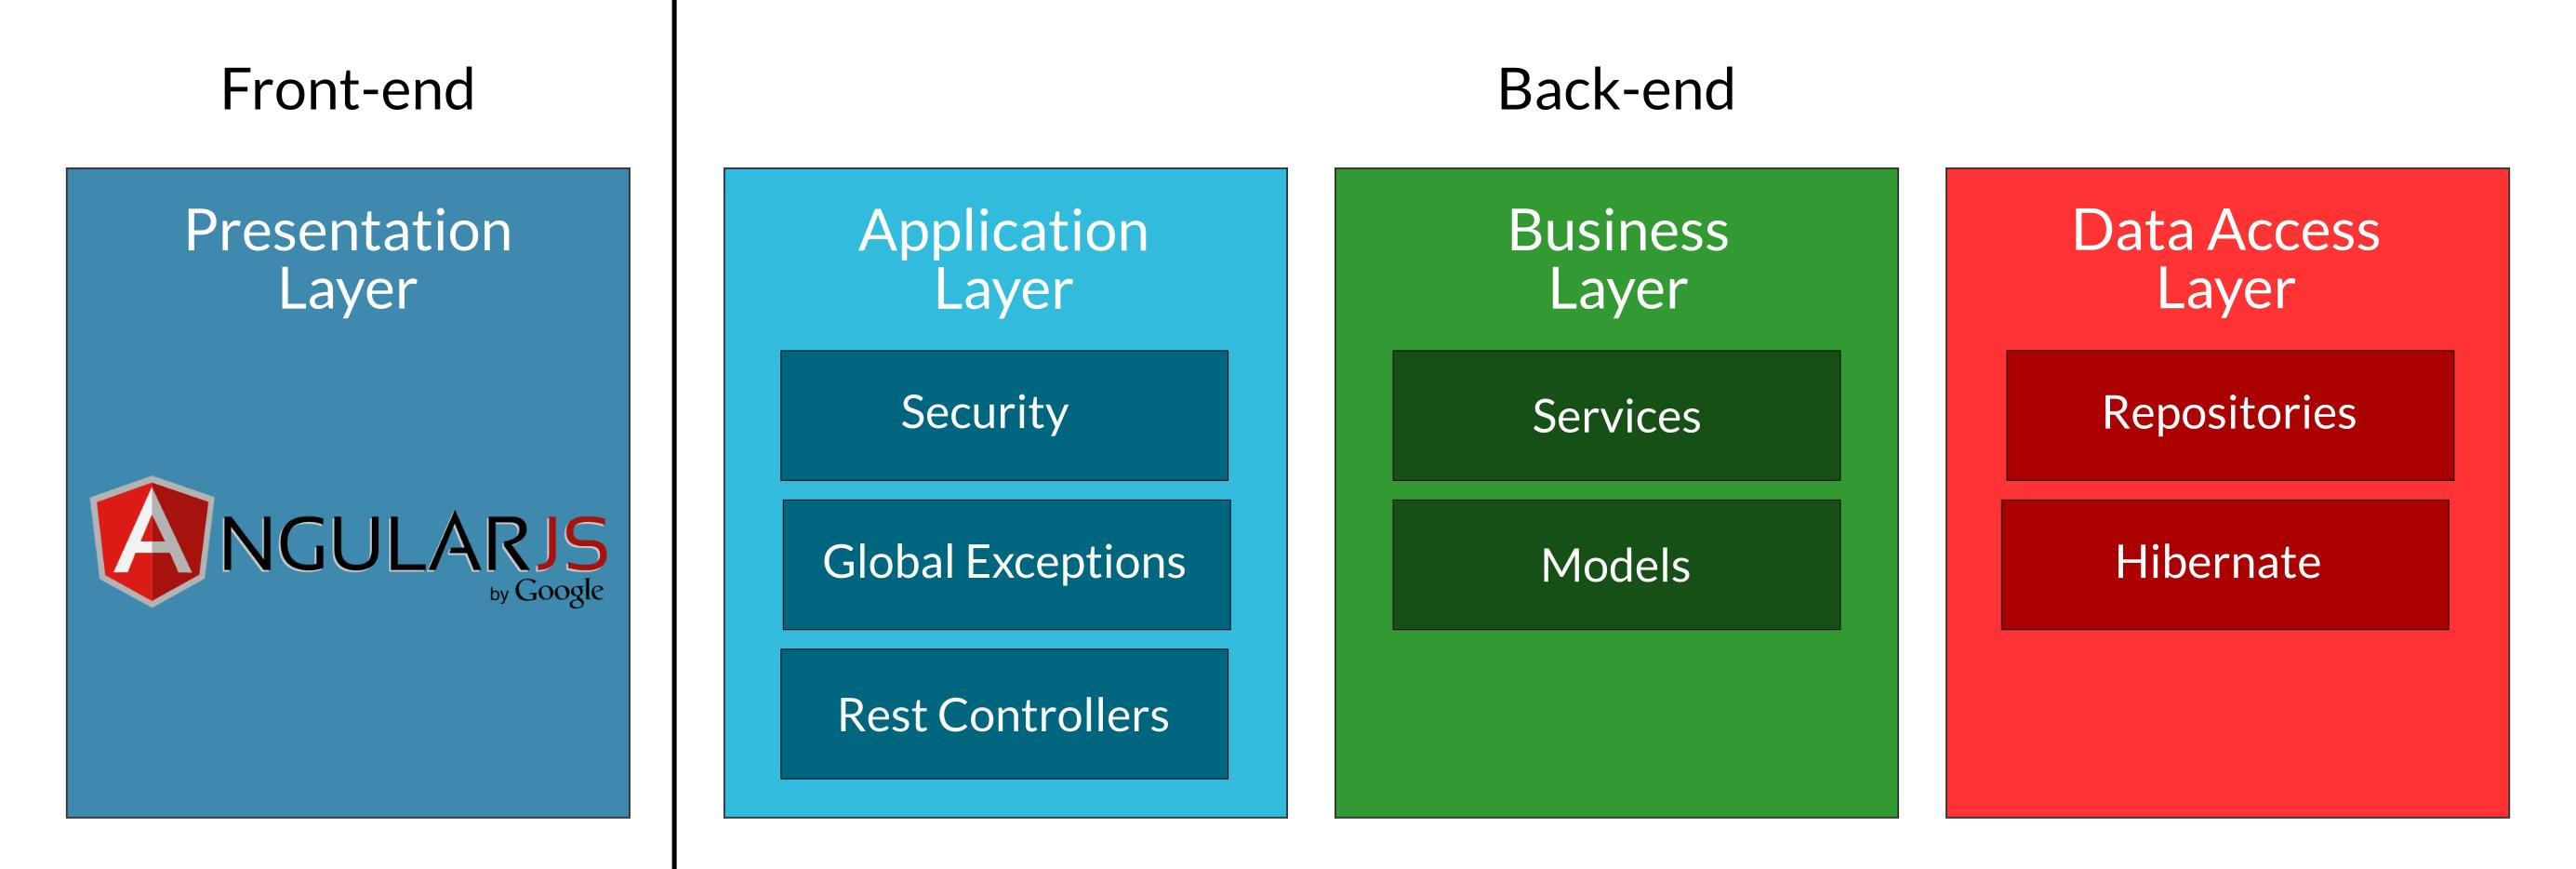
\includegraphics[width=0.80\textwidth]{architecture-layer}}
	\caption{Architecture: Multilayer architecture}
	\label{fig:architecture-layer}
\end{figure}

Our layers depend on each other while every layer communicates only with either the upper (consumer) or the lower (service provider) layer. This ensures a good maintainability and loose coupling of the single layers.\newline
At this point an example should be given: If the \textit{presentation layer} needs to display an expense, the \textit{application layer} will handle this request by first checking the relevant security parameter of the request followed by calling the \textit{business layer}. The \textit{business layer} will handle and aggregate the desired information fetched from the relevant models. In our case to display an expense, the service will retrieve all expense-items and expense-item-attachments from the database using the \textit{data access layer}. Since the \textit{data access layer} provides a uniform interface, the \textit{business layer} does not care if a H2 or Postgres database is used - it just calls the interface and gets the information. The \textit{business layer} passes the data to the \textit{application layer}, where it is serializes as JSON and sent as request-response to the \textit{presentation layer}. There, the data is processed and displayed in the GUI.

\subsection{Back-end}
The back-end is developed in Java. It is structured according to the rules of a multilayered software architecture. We use the domain driven design \cite{ddd} to apply common patterns for the layers in the back-end. The domain model, that consists of the concepts, is connected to the database. Changes on the model will be automatically synchronized with the database. The service package lists all methods that are used on a domain model.\newline
DTOs (Data Transfer Object) are used to transfers data from back-end to front-end and vice verse. \newline The implemented model- and service-classes are visualized in appendix \ref{sec:app-models} and \ref{sec:app-service}. \par



\subsection{Front-end}
The front-end is developed in JavaScript using the AngularJS framework\cite{angular}. AngularJS is based on a MVC (Model View Controller) pattern. It basically consists of controllers, templates that are used for the view  as well as models representing the data that is shown to the user using the templates. However, AngularJS  extends the basic MVC concept with useful enhancements like directives, filters, injectors etc. A complete list of the available concepts in AngularJS can be found in the AngularJS Developer Guide \cite{angular-devguide}.

\section{Technologies}

In the following section the technologies used are described and explained why they were chosen.

\subsection{Back-end}

\subsubsection{Java}
The reimbursement-tool uses for the back-end part Java SE 7. Java is a mature programming language developed and maintained by Oracle\cite{java}, has detailed documentation and since Java is taught at IFI's Info 1 course, an adequate support and further development of the reimbursement tool can be guaranteed.

\subsubsection{Hibernate}
\textit{Hibernate} abstracts the data layer. So that SQL-queries have to be written in rare cases only, which increases the code-clarity and decreases the code-complexity. All data operation are handled implicitly by defined Java data classes.\newline
H2 database is a temporary database for storing data in a database environment. It offers a simple interface and can be used for development, given that only one development database server is available. \cite{hibernate}

\subsubsection{Spring Framework}
We decided to use the \textit{Spring Framework}\cite{spring} because it's well documented, widely used and easy to integrate in an existing Java project. Therefore we use various components and sub-packages of Spring. These are:
\begin{itemize}
	\item Spring Security for the login- and user-management as well as role based access-management for the RESTful resources.
	\item Spring Web MVC is used to define RESTful interface within a few lines of code.
	\item Spring ORM used for the XML mapping within the process of Pdf-generation.
	\item Spring Data is used to provide a simpler method to use data access technologies. It uses the DAO (Data Access Object) \cite{dao} to access data in a standard database like SQL.
	\item Spring Test and Spring Security Test provide means for a convenient integration testing.
\end{itemize}

\subsubsection{Maven}
The tool uses Apache Maven \cite{maven} for the build process and dependency management. We decided to use it, because it is widely used and is easy to maintain with a single \textit{pom.xml} file.

\subsubsection{Apache FOP}
The generated Pdf by the reimbursement-tool needs to be identical to the existing MS-Office Excel-Pdf file provided by the Finance Administration of the University of Zurich. The generated Pdf structure is added in \ref{sec:app-pdf}.\newline
The Pdf gets generated using an individual created XSLT template and a XML document generated out of a Java Object. Combining these two files generates an \textit{.fo} document, which will be used by Apache FOP \cite{apache-fop} to generate the Pdf.\par
We decided for Apache FOP because it is based on widely used standards like XML and XSL so that ongoing maintenance can be achieved easily and without specific knowledge required.

\subsubsection{Pdfsign.js}
The ability to sign the printed Pdf document is crucial so that authenticity is guaranteed. Especially if the Pdf document will be used as evidence by the Finance Administration of the University of Zurich. The system provides two types of signatures \cite{arx-signature}:
\begin{itemize}
	\item A \textbf{Digital signature} ensure the authenticity of the signer. Any changes made to the document after it has been signed will invalidate the signature. To use it the user has to provide his private key to successfully sign the document.
	\item \textbf{Electronic signature} does not ensure the authenticity of the signer. Anyone can theoretically make changes on the document after it has been signed without the signature become invalid. Of course, in our tool this is prevented by design. The handwritten signature captured during the registration will be stamped on the Pdf document.
\end{itemize}\par

The implementation of the digital signature is done using a third party library pdfsign.js \cite{pdfsign} that allows us to do the pdf signing in the browser and not on the server. Due to the requirement, that the private key cannot be uploaded or processed by the server, the signing needs to be done on the client using the web browser.\par

All involved participants need to sign the document; \textit{Expense Creator}, \textit{Manager} and the \textit{Finance administration} to proof their acceptance of the expense and the captured receipts. \par

\subsubsection{Public Interface}

\paragraph{RESTful API}
\label{sec:restfulapi}
The tool uses a RESTful API that provides services to access the back-end resources. It is implemented using the Spring MVC. /newline
The available methods provided by the back-end are listed in \ref{sec:rest-services}. There exist private and public services. Private services can only be access by a \textbf{Registered user / User} (private services are marked with the term PRIVATE).

\paragraph{Swagger UI}
The Swagger UI visualizes all methods provided by the RESTful interface using a simple GUI. Furthermore developers can interact directly with the Swagger UI to test the \texttt{HTTP} methods. Figure \ref{fig:swagger01} shows a screen-shot of our Swagger UI. It visualizes all the available methods for the \texttt{public} resource as well as the mandatory and optional parameters for \texttt{HTTP} calls. This was important for the process of development. \cite{swagger} \par
We decided on Swagger UI, because a simple and easy to understand overview, as well as a simple integration into the software source-code. Further testing the back-end functionality was very simple using Swagger UI.

\begin{figure}[H]
	\centering
	\fbox{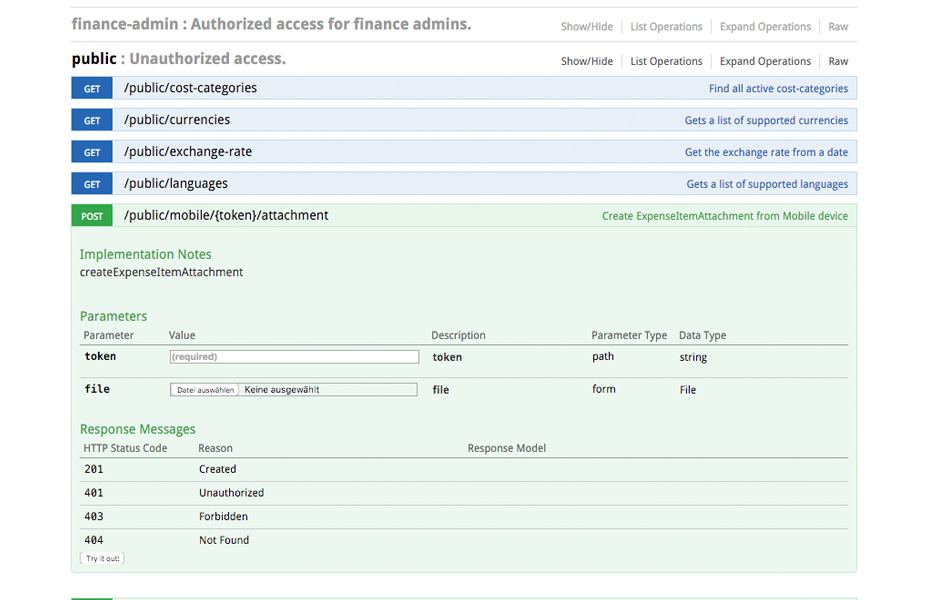
\includegraphics[width=0.80\textwidth]{swagger01}}
	\caption{Swagger: Reimbursement GUI}
	\label{fig:swagger01}
\end{figure}

\subsection{Front-end}

\subsubsection{AngularJS}
The tool uses the AngularJS framework. Its data bindings and dependency injections reduces the amount of code need to be written. Further it uses HTML templates and an sophisticated routing concept to deliver interactive GUIs. AngularJS is based on an MVC approach and is easy to integrate with REST services.\cite{angular}\par
We used AngularJS because of its broad community and the fact that it's supported by Google makes it future-proof.

\subsubsection{Bootstrap}
Bootstrap is a framework that consists of HTML, CSS and JavaScript elements. It can be used to create appealing responsive websites. Further it's CSS elements are supported by most of the desktop and mobile web-browsers available. The tool uses Bootstrap v. 3.3.5. \cite{bootstrap}\par
We use Bootstrap to speed-up the GUI development process. Using the elements it provides makes it easy to setup a responsive website within minutes. Further it provides a lot of fancy HTML/CSS elements like \textit{accordions}, \textit{modals}, etc.

\subsubsection{Bower}
The tool uses Bower for the client-side package management. Bower is a package manager for JavaScript web applications like AngularJS. It keeps track of the used assets, frameworks, libraries, etc. \cite{bower} \par
We used Bower because of its widely used, has a sound documentation and is easy to work with.

\subsubsection{Grunt}
Grunt is a JavaScript task runner. We use it for our client-side build. Its plugin directory supports a lot of modules to optimize the development work flow. Code-uglifying, concatenating, sass-compiling, file operations, auto prefixing etc. \cite{grunt} \par
We used Grunt because its widely used and there exists sound know how about its usage in our team.



\section{Testing}

\subsection{Unit Testing}
Since the application is quite big in scope, the unit testing has in accordance with the supervisors been neglected. To still ensure a high software quality, integration tests are preferred.

\subsection{Integration Testing}
To detect the impact of code changes, integration tests cover the main scenarios. These are:
\begin{itemize}
	\item Registration
	\item Login
	\item Expense Creation
	\item Expense Item Creation
	\item Attachment upload
	\item Assigning of expenses to IFI Finadmins
	\item Validation of Expenses (Managers and IFI Finadmins)
	\item Digitally Signing
	\item End-To-End Process for Assistant-Prof-Finadmin-Assistant-Prof-Finadmin
	\item End-To-End Process for Prof-Finadmin-Prof-Depman-Finadmin
	\item End-To-End Process for Finadmin-Finadmin2-Finadmin-Depman-Finadmin2
	\item End-To-End Process for Depman-Finadmin-Depman-Headinst-Finadmin
	\item End-To-End Process for Headinst-Finadmin-Headinst-Depman-Finadmin
\end{itemize}


\subsection{Load Testing}
The reimbursement tool has been load-tested using the tools JMeter\cite{jmeter} in combination with VisualVM\cite{visualvm}.

\paragraph{Apache JMeter} "JMeter is an open source software designed to load test functional behavior and measure performance. It was originally designed for testing Web Applications but has since expanded to other test functions."\cite{jmeter}.\par

In JMeter, all required steps to perform a document upload have been modelled and compiled into a testsuite.

\paragraph{VisualVM} "VisualVM is a visual tool integrating several commandline JDK tools and lightweight profiling capabilities. Designed for both production and development time use, it further enhances the capability of monitoring and performance analysis for the Java SE platform."\cite{visualvm}.\par 
VisualVM enables the live monitoring of the active configuration, heap space, classes, instances and tasks running on the VM, where the application is deployed.\par

To retrieve and display information on applications running on the remote host, the \textbf{jstatd} utility needs to be running on the remote host. Additionally a security policy file must be in place. We prepared our VMs to have the security policy file present in the \textbf{jstatd} folder:  \textit{/usr/lib/jvm/java-7-openjdk-amd64/bin/jstatd.all.policy}.\par

How to start monitorng:
\begin{itemize}
	\item SSH to the VM, in our example the INT VM
	\item in one command: "\textit{sudo jstatd -J-Djava.security.policy=/usr/lib/jvm/java-7-openjdk-amd64/bin/jstatd.all.policy -J-Djava.rmi.server.hostname= \textbf{HOST\_IP\_ADDRESS}}"
	\item Switch back to your own computer and start VisualVM: it’s located in the Java/JDK/bin folder and is called \textbf{jvisualvm.exe}
	\item "File" - "Add Remote": Host: 192.41.136.227, Name: whatever you like
	\item Security note: Watch out to kill the \textbf{jstatd} process manually (kill PID) if the process is not killed on logout or if the terminal looses connection.
\end{itemize}

\paragraph{Findings}
The load tests have shown, that the conversion of large images could cause a bottleneck. Since the image-formats are converted to PDF only on the back-end, large images consume a huge amount of the available heap. With 2gb heap space, only 6 parallel uploads of 8mb large images can be handled. A possible work-around would be to convert the images already on the client to pdf-format and only send the pdf-documents to the server.\par

Another potential bottleneck could arise, if large amounts of expenses are in the dashboard. In this case, the back-end would serialize all data required to display these expenses in a single request. This could be mitigated by implement pagination i.e. chunks of N expenses are sent to the client. If more expenses are required, the back-end sends the second page, namely the second chunk of N expenses.

\subsection{User and GUI Testing}
The graphical user interface is simple and practical. Nevertheless it provides a good user guidance and pleases the eye with subtle animations.\par

The user interface of the front-end has been tested through the supervisors and Claudia Leibundgut and has been improved over numerous iterations. Since no business logic is present in the front-end, and the back-end handles all security relevant concerns, the programmatical testing of the front-end has been neglected.
